\begin{frame}[fragile]
\frametitle{Innovación}
\begin{table}
\begin{tabular}{p{7cm}p{3cm}}
\small
\begin{verbatim}
«La innovación por la innovación no sirve para nada.
Innovar es crear productos que hagan la vida más fácil.»
\end{verbatim}&\\
\normalsize
\begin{itemize}
    \item Creación o modificación de un producto y su introducción en un
    mercado.
    \item Renovar, introducir una novedad.
\end{itemize}
&
\vspace{1cm}
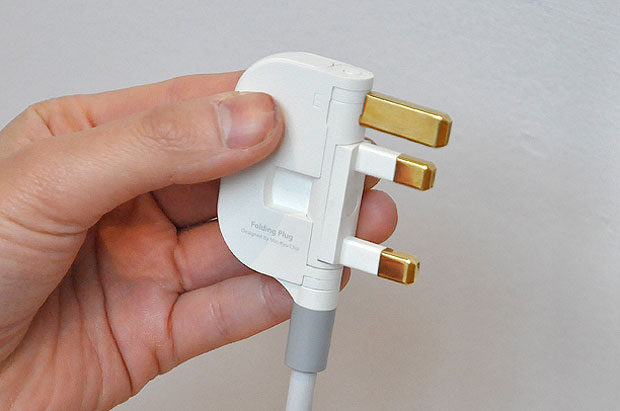
\includegraphics[width=4cm]{img/enchufe.jpg}\\
\end{tabular}
\end{table}
\end{frame}

